\documentclass[
	10pt,								% globale Schriftgröße
	parskip=half-,						% setzt Absatzabstand hoch
	paper=a4,							% Format
	english,ngerman,					% lädt Sprachpakete
	]{scrartcl}							% Dokumentenklasse

% //////////////////// Pakete laden ////////////////////
\usepackage[fleqn]{amsmath}
\usepackage[fleqn]{mathtools}
\usepackage{amssymb}			% mathematische symbole, für \ceckmarks
\usepackage{amsthm}				% für proof
\usepackage{mathrsfs}			% für \mathscr
\usepackage{latexsym}
\usepackage{marvosym}				% für Lightning

\usepackage{fontspec} 			% funktioniert nur mit den neueren Compilern z.B. XeLaTeX
\usepackage{microtype}			% für bessere Worttrennung
\usepackage[ngerman]{babel} 	% Spracheinstellung
\usepackage{lmodern}			% verändert verwendete Schriftart, damit sie weniger pixelig ist

\usepackage{verbatim}
\usepackage{listings}			% Für Quellcode

\usepackage{graphicx}
\usepackage{tabularx}			% für Tabellen mit gleicher Spaltenbreite und automatischen Umbrüchen
\usepackage{fullpage}
\usepackage{multirow}			% für multirow in tabulars
\usepackage{rotate}
\usepackage[cmyk,table]{xcolor} % um Farben zu benutzen, kann mehr als das Paket color
\usepackage[					% Verlinkungen
	colorlinks,					% farbige Schrift, statt farbiger Rahmen
	linktocpage,				% verlinkt im Abb.Verzeichnis Seitenzahl statt Bildunterschrift
	linkcolor=blue				% setzt Farbe der Links auf blau
	]{hyperref}					% nur für digitale Anwendungen, url = "http://www.example.com"
\usepackage{url}				% für Webadressen wie e-mail usw.: "\url{http://www.example.com}"

\usepackage{enumerate}			% für versch. Aufzählungezeichen wie z.B. a)
\usepackage{xspace}				% folgt ein Leerzeichen nach einem \Befehl, wird es nicht verschluckt.
\usepackage{cancel}				% für das Durchstreichen u.a. in Matheformeln mit \cancel
\usepackage{float}              % zum Forcieren der Position von figure-Umgebungen

% zum Zeichnen (u.a. von Graphen)
\usepackage{fp}
\usepackage{tikz}
\usetikzlibrary{tikzmark}			% für \tikzmark{toRemember}
\usetikzlibrary{positioning}	% verbesserte Positionierung der Knoten
\usetikzlibrary{automata}		% für Automaten (GTI)
\usetikzlibrary{arrows}
\usetikzlibrary{shapes}
\usetikzlibrary{decorations.pathmorphing}
\usetikzlibrary{decorations.pathreplacing}
\usetikzlibrary{decorations.shapes}
\usetikzlibrary{decorations.text}

% //////////////////// Syntaxhighlighting ////////////////////
\lstloadlanguages{Python, Haskell, [LaTeX]TeX, Java}
\lstset{
   basicstyle=\footnotesize\ttfamily,	% \scriptsize the size of the fonts that are used for the code
   backgroundcolor = \color{bgcolour},	% legt Farbe der Box fest
   breakatwhitespace=false,	% sets if automatic breaks should only happen at whitespace
   breaklines=true,			% sets automatic line breaking
   captionpos=t,				% sets the caption-position to bottom, t for top
   commentstyle=\color{codeblue}\ttfamily,% comment style
   frame=single,				% adds a frame around the code
   keepspaces=true,			% keeps spaces in text, useful for keeping indentation
							% of code (possibly needs columns=flexible)
   keywordstyle=\bfseries\ttfamily\color{codepurple},% keyword style
   numbers=left,				% where to put the line-numbers;
   							% possible values are (none, left, right)
   numberstyle=\tiny\color{codegreen},	% the style that is used for the line-numbers
   numbersep=5pt,			% how far the line-numbers are from the code
   stepnumber=1,				% nummeriert nur jede i-te Zeile
   showspaces=false,			% show spaces everywhere adding particular underscores;
							% it overrides 'showstringspaces'
   showstringspaces=false,	% underline spaces within strings only
   showtabs=false,			% show tabs within strings adding particular underscores
   flexiblecolumns=false,
   tabsize=1,				% the step between two line-numbers. If 1: each line will be numbered
   stringstyle=\color{orange}\ttfamily,	% string literal style
   numberblanklines=false,				% leere Zeilen werden nicht mitnummeriert
   xleftmargin=1.2em,					% Abstand zum linken Layoutrand
   xrightmargin=0.4em,					% Abstand zum rechten Layoutrand
   aboveskip=2ex, 
}

\lstdefinestyle{py}{
   language=Python,
}
\lstdefinestyle{hs}{
   language=Haskell,
}
\lstdefinestyle{tex}{
	language=[LaTeX]TeX,
	escapeinside={\%*}{*)},     % if you want to add LaTeX within your code
	texcsstyle=*\bfseries\color{blue},% hervorhebung der tex-Schlüsselwörter
	morekeywords={*,$,\{,\},\[,\],lstinputlisting,includegraphics,
	rowcolor,columncolor,listoffigures,lstlistoflistings,
	subsection,subsubsection,textcolor,tableofcontents,colorbox,
	fcolorbox,definecolor,cellcolor,url,linktocpage,subtitle,
	subject,maketitle,usetikzlibrary,node,path,addbibresource,
	printbibliography},% if you want to add more keywords to the set
     numbers=none,
     numbersep=0pt,
     xleftmargin=0.4em,
}

\lstdefinestyle{java}{
	language=Java,
	extendedchars=true,		% lets you use non-ASCII characters;
   						% for 8-bits encodings only, does not work with UTF-8
}

\lstdefinelanguage[x64]{Assembler}     % add a "x64" dialect of Assembler
   [x86masm]{Assembler} % based on the "x86masm" dialect
   % with these extra keywords:
   {morekeywords={CDQE,CQO,CMPSQ,CMPXCHG16B,JRCXZ,LODSQ,MOVSXD, %
                  POPFQ,PUSHFQ,SCASQ,STOSQ,IRETQ,RDTSCP,SWAPGS, %
                  rax,rdx,rcx,rbx,rsi,rdi,rsp,rbp, %
                  r8,r8d,r8w,r8b,r9,r9d,r9w,r9b}
}					% for 8-bits encodings only, does not work with UTF-8

\lstdefinestyle{c}{
	language=c,
	extendedchars=true,		% for 8-bits encodings only, does not work with UTF-8
}

% //////////////////// eigene Kommandos ////////////////////
\newcommand\FU{Freie Universität Berlin\xspace}% benötigt package xspace
\newcommand\gdw{g.\,d.\,w.\xspace}
\newcommand\oBdA{o.\,B.\,d.\,A.\xspace}
\newcommand{\Eu}{\texteuro}
\newcommand\N{\mathbb{N}\xspace}
\newcommand\Q{\mathbb{Q}\xspace}
\newcommand\R{\mathbb{R}\xspace}
\newcommand\Z{\mathbb{Z}\xspace}
\newcommand\ohneNull{\ensuremath{\backslash\lbrace 0\rbrace}}% \{0}
\let\dhALT\dh	% Schreibt Befehl \dh in \dhALT um
\renewcommand\dh{d.\,h.\xspace}	%renew überschreibt command \dh
\newcommand\Bolt{\;\text{\LARGE\raisebox{-0.3em}{\Lightning}\normalsize}\xspace}% Blitz
\newcommand\zz{\ensuremath{\raisebox{+0.25ex}{Z}% zu zeigen
			\kern-0.4em\raisebox{-0.25ex}{Z}%
			\;\xspace}}
\newcommand{\from}{\ensuremath{\colon}}
\newcommand{\floor}[1]{\lfloor{#1}\rfloor}
\newcommand{\ceil}[1]{\lceil{#1}\rceil}
 \renewcommand{\L}{\ensuremath{\mathcal{L}}\xspace}
 \renewcommand{\P}{\ensuremath{\mathcal{P}}\xspace}
 \newcommand{\NL}{\ensuremath{\mathcal{N}\kern-0.2em\mathcal{L}}\xspace}
 \newcommand{\NP}{\ensuremath{\mathcal{NP}}\xspace}

% //////////////////// Mathefunktionen ////////////////////
\DeclareMathOperator{\Landau}{\mathcal{O}}
\DeclareMathOperator{\True}{True}
\DeclareMathOperator{\False}{False}

% //////////////////// eigene Theoreme ////////////////////
\newtheorem{theorem}{Satz}
\newtheorem{corollary}[theorem]{Folgerung}
\newtheorem{lemma}[theorem]{Lemma}
\newtheorem{observation}[theorem]{Beobachtung}
\newtheorem{definition}[theorem]{Definition}
\newtheorem{Literatur}[theorem]{Literatur}
% konfiguriert proof
\makeatletter
\newenvironment{Proof}[1][\proofname]{\par
  \pushQED{\qed}%
  \normalfont \topsep6\p@\@plus6\p@\relax
  \trivlist
  \item[\hskip\labelsep
%         \itshape
        \bfseries
    #1\@addpunct{.}]\ignorespaces
}{%
  \popQED\endtrivlist\@endpefalse
}
\makeatother

% //////////////////// eigene Farben ////////////////////
\let\definecolor=\xdefinecolor
\definecolor{FUgreen}{RGB}{153,204,0}
\definecolor{FUblue}{RGB}{0,51,102}

\definecolor{middlegray}{rgb}{0.5,0.5,0.5}
\definecolor{lightgray}{rgb}{0.8,0.8,0.8}
\definecolor{orange}{rgb}{0.8,0.3,0.3}
\definecolor{azur}{rgb}{0,0.7,1}
\definecolor{yac}{rgb}{0.6,0.6,0.1}
\definecolor{Pink}{rgb}{1,0,0.6}

\definecolor{bgcolour}{rgb}{0.97,0.97,0.97}
\definecolor{codegreen}{rgb}{0,0.6,0}
\definecolor{codegray}{rgb}{0.35,0.35,0.35}
\definecolor{codepurple}{rgb}{0.58,0,0.82}
\definecolor{codeblue}{rgb}{0.4,0.5,1}

% //////////////////// eigene Settings ////////////////////

\textheight = 230mm		% Höhe des Satzspiegels / Layouts
\footskip = 10ex			% Abstand zw. Fußzeile und Grundlinie letzter Textzeile
\parindent 0pt			% verhindert Einrückung der 1. Zeile eines Absatzes
\setkomafont{sectioning}{\rmfamily\bfseries}% setzt Ü-Schriften in Serifen, {disposition}											% bindet Header ein (WICHTIG)
\usepackage{graphicx}
\usepackage{amsmath}
\usepackage{amssymb}
\usepackage{fancyvrb}

\newcommand{\dozent}{Prof. R. Rojas}					% <-- Names des Dozenten eintragen
\newcommand{\projectNo}{9}
\newcommand{\veranstaltung}{Mustererkennung}
\newcommand{\semester}{WS17/18}
\newcommand{\studenten}{Boyan Hristov, Nedeltscho Petrov}
% /////////////////////// BEGIN DOKUMENT /////////////////////////


\begin{document}
% /////////////////////// BEGIN TITLEPAGE /////////////////////////
\begin{titlepage}
	\subject{\dozent}
	\title{\veranstaltung, \semester}
	\subtitle{\Large Übungsblatt \projectNo\\ \large\vspace{1ex} }
	\author{\studenten}
	\date{\normalsize \today}
\end{titlepage}

\maketitle								% Erstellt das Titelblatt
\vspace*{-9cm}							% rückt Logo an den oberen Seitenrand
\makebox[\dimexpr\textwidth+1cm][r]{	%rechtsbündig und geht rechts 1cm über Layout hinaus
	
\includegraphics[width=0.4\textwidth]{src/fu_logo} % fügt FU-Logo ein
}
% /////////////////////// END TITLEPAGE /////////////////////////

\vspace{7cm}							% Abstand
\rule{\linewidth}{0.8pt}				% horizontale Linie										% erstellt die Titelseite


Link zum Git Repository: \url{https://github.com/BoyanH/FU-MachineLearning-17-18/tree/master/Solutions/Homework\projectNo}

\section*{Neural Networks}
Wir haben zwei Implementierungen - eine mit streng nur 1 hidden Layer und eine, die als Argument ein Tupel, dass
die Anzahl von Neuronen pro Layer beschreibt und damit auch die Anzahl von layers. Die komplexere Implementierung
ist aber deutlich weniger lesbar und viel zu schwierig einzustellen.
Deswegen werden wir uns hier auf die Beschreibung unserer simpleren Implementierung konzentrieren. Beide Implementierungen
sind am Ende des Blattes zu sehen.

\section*{Evaluation}
Die Methode ist, wie man später anhand der booleschen Funktionen sieht, viel mächtiger, aber auch viel schwieriger
einzustellen. Wir haben eine Fehlerrate von knapp über 11\% bekommen, was eigentlich sehr schlecht ist. Wir denken aber,
dass das eher an der Lernrate und Anzahl von Neuronen / Schichten im Netz hängt. Die Methode ist auch sehr aufwändig
im Sinne von Rechnerressourcen, wie aber im Tutorial beschrieben, könnte diese effizient in Hardware implementiert
werden. Wenn wir aber uns entschieden sollen für diesen Datensatz (Ziffererkennung) wurden wir eher eine lineare
Methode nehmen, die viel schneller ist und leichter zu interpretieren. Wir haben aber immer noch Hoffnung, dass wir
bessere neuronale Netze implementieren werden. \\ \\

Wie wir auf der offizieler Seite des Datensatz gesehen haben, benutzt man echt viele hidden Layers um die
Daten gut zu klassifizieren. Leider sind beide unsere Implementierung und Rechnern nicht so perfekt für solche
Ansätze.

\section*{Fehler über die Iterationen}

\section*{1 Hidden Layer mit 15 Neuronen}

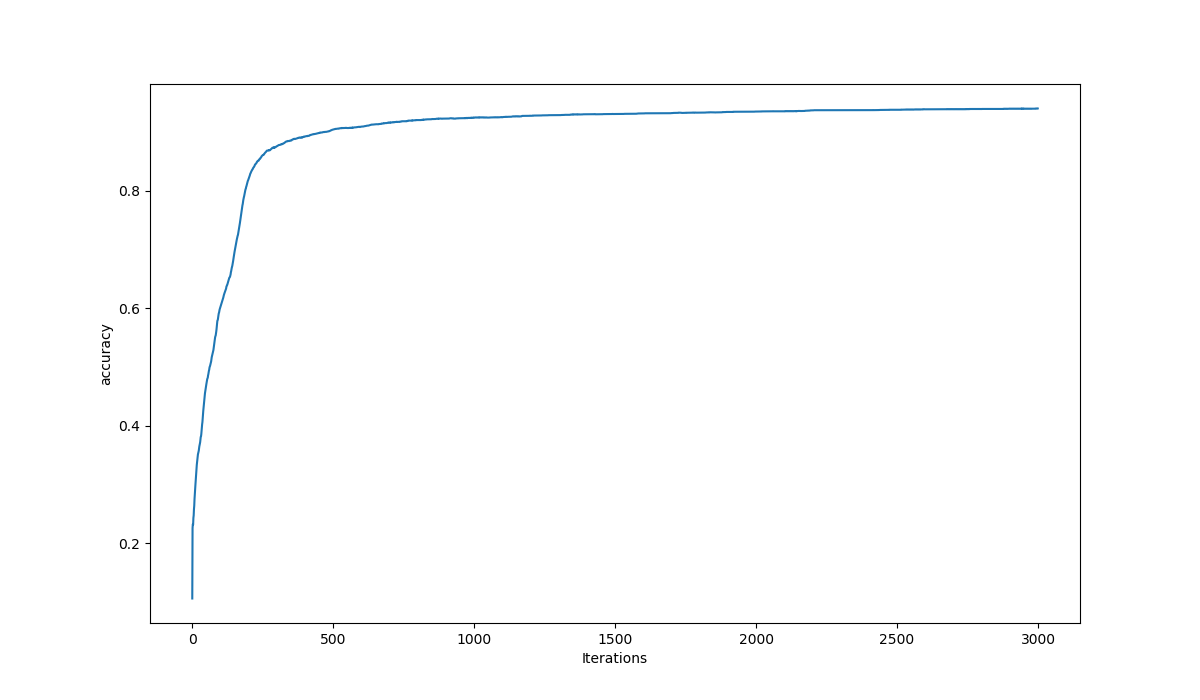
\includegraphics[height=8cm]{./15inner.png}

Output: \\
Score: 0.88458781362

\section*{1 Hidden Layer mit 20 Neuronen}

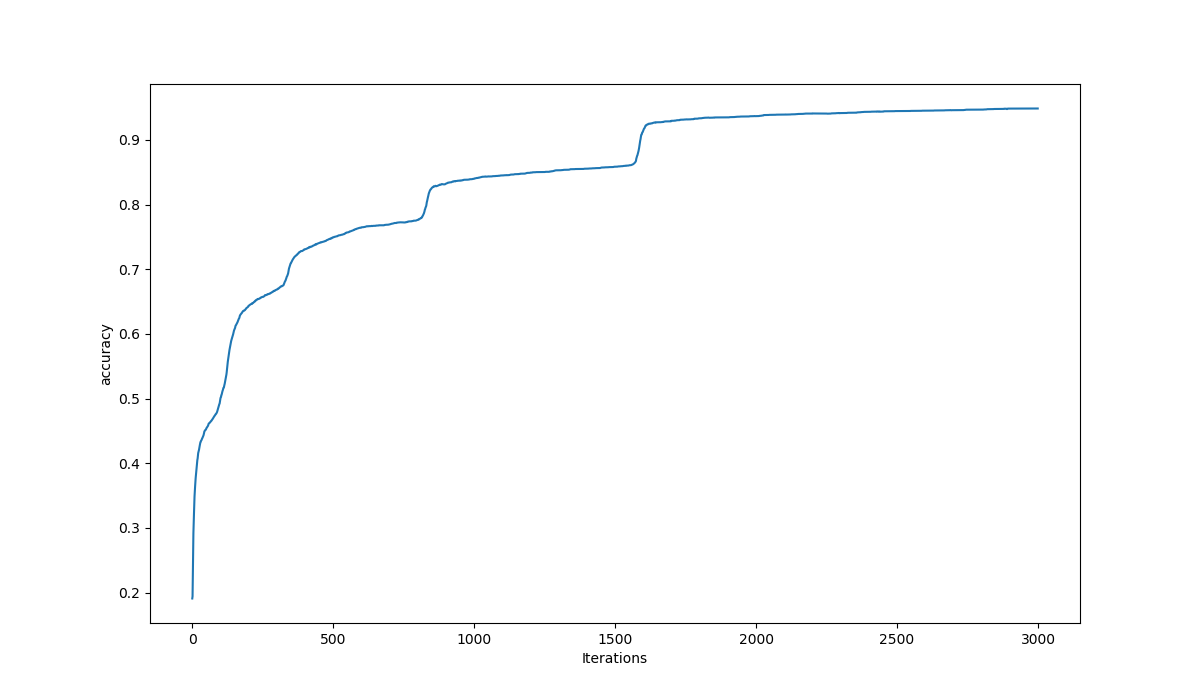
\includegraphics[height=8cm]{./20inner.png}

Output: \\
Score: 0.8863799283154122 \\
Score train: 0.9512907191149355

\section*{1 Hidden Layer mit 25 Neuronen}

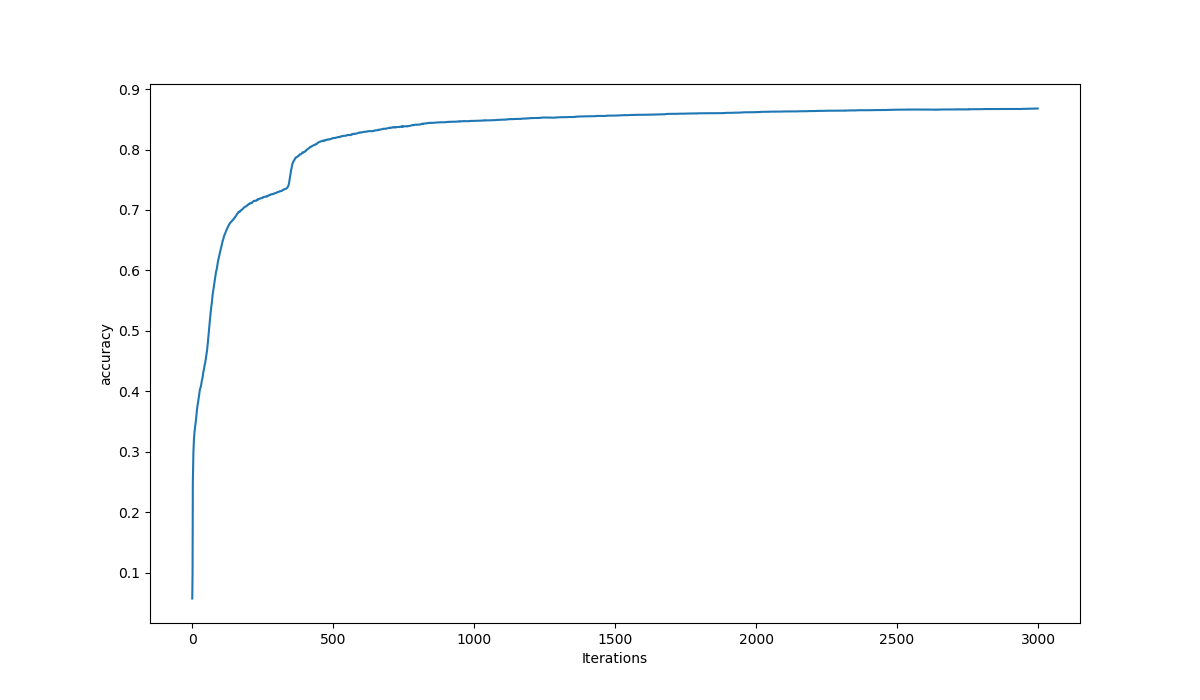
\includegraphics[height=8cm]{./25inner.png}

Output: \\
Score train: 0.8678549477566072 \\
Score: 0.8182795698924731

\section*{2 Hidden Layers mit 20 und 15 Neuronen, circa 7 Batches (max. 1000 Beispiele pro Batch)}
Wir wurden gerne noch mehr mit mehreren Schichten spielen, das war aber viel zu rechenaufwändig...


Wie man aber hier sieht, haben wir bei den Testdatensatz besseres Score als bei den Trainingsdatesatz,
was ein sehr gutes Zeichen in Richtung "nicht auswendig lernen" ist. Yey :)

Output
\begin{lstlisting}
Score train: 0.7744314689612785
Score: 0.7548387096774194

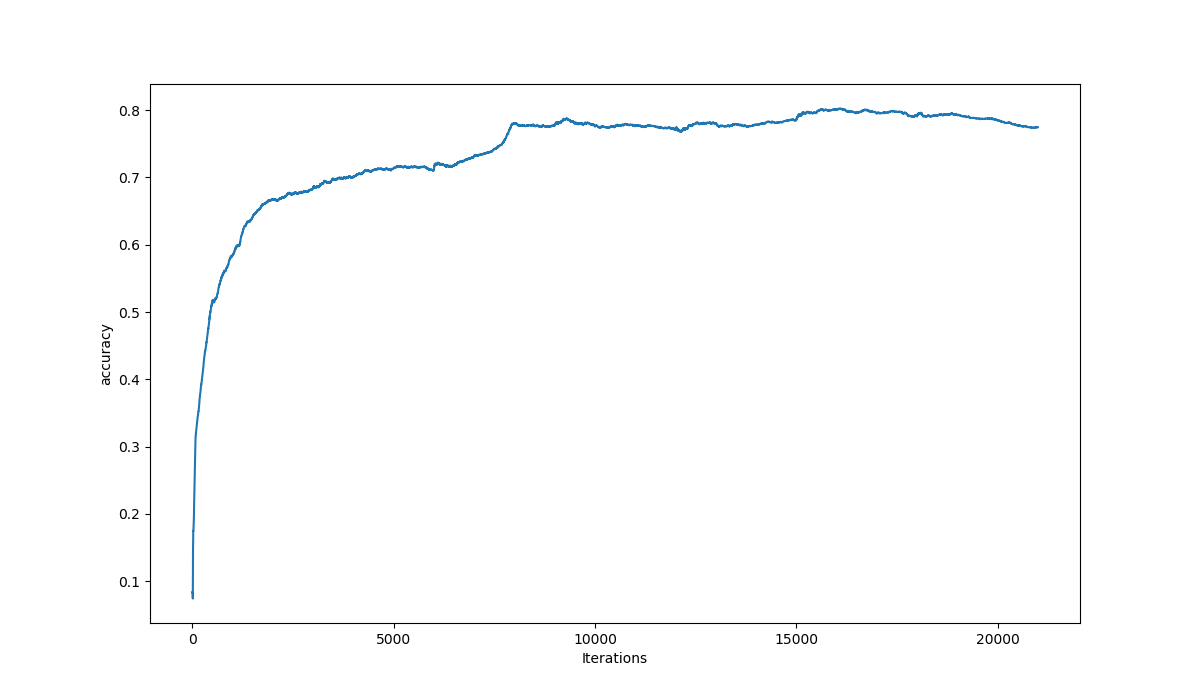
\includegraphics[height=8cm]{./2_hidden_layers_20_15_with_7_batches.png}

\end{lstlisting}

\section*{1 Hidden Layer, 20 Neuronen, großen Datensatz}
Leider müssten wir den Code von NN.py noch etwas ändern, damit wir eine vernünftige Laufzeit kriegen. Wir haben
batches eingefügt und auch einstellbare Anzahl von Beispiele pro Batch. Dazu müssten wir leider nur den Score
innerhalb des Batches plotten lassen, sonst dauert eine Prediction innerhalb der Iterationsschleife viel zu lange.
Unsere Methode ist für den großen Datensatz gar nicht optimal, da es lange Zeit braucht zum Ausführen
könnten wir es nicht viel optimieren. \\

Da das kleine Datensatz nur etwas über 6 tausend Beispiele hat, ist das Plotting da immer noch korrekt mit der ganzen
Fehler bei der Trainingsdatensatz. \\

Hier wurden auch nur 250 Iterationen pro Batch gemacht, also das ganze ist weit weg von präzise, wir wollten aber
schauen was für Ergebnisse man bekommt mit dem großen Datensatz, wenn man mehrere unterschiedliche Beispiele sieht und
weniger dabei korrigiert.\\

Output

\begin{lstlisting}
fetching data-set
MNIST original fetched
#Batches: 49
#Iterations per batch: 250
Batch #1 completed!
Batch #2 completed!
Batch #3 completed!
Batch #4 completed!
Batch #5 completed!
Batch #6 completed!
Batch #7 completed!
Batch #8 completed!
Batch #9 completed!
Batch #10 completed!
Batch #11 completed!
Batch #12 completed!
Batch #13 completed!
Batch #14 completed!
Batch #15 completed!
Batch #16 completed!
Batch #17 completed!
Batch #18 completed!
Batch #19 completed!
Batch #20 completed!
Batch #21 completed!
Batch #22 completed!
Batch #23 completed!
Batch #24 completed!
Batch #25 completed!
Batch #26 completed!
Batch #27 completed!
Batch #28 completed!
Batch #29 completed!
Batch #30 completed!
Batch #31 completed!
Batch #32 completed!
Batch #33 completed!
Batch #34 completed!
Batch #35 completed!
Batch #36 completed!
Batch #37 completed!
Batch #38 completed!
Batch #39 completed!
Batch #40 completed!
Batch #41 completed!
Batch #42 completed!
Batch #43 completed!
Batch #44 completed!
Batch #45 completed!
Batch #46 completed!
Batch #47 completed!
Batch #48 completed!
Batch #49 completed!
Score train: 0.8551020408163266
Score: 0.8544761904761905

\end{lstlisting}

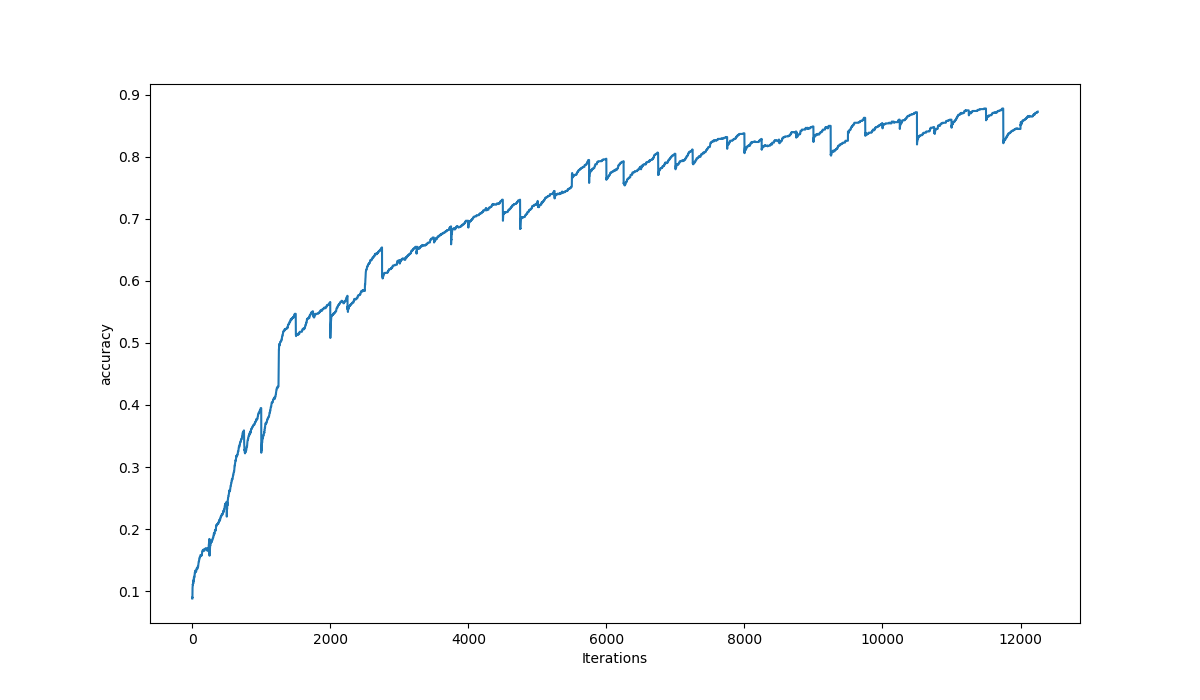
\includegraphics[height=8cm]{./20_inner_big.png}

Wie man auf dem Plot sieht, senkt das Score wenn ein neues Batch eingefügt wird, da wir diese Beispiele noch nie
gesehen haben. Dann wird die Korrektur bei den Gewichtsmatritzen gemacht und den Score steigt wieder.
Ein Score von 85\% finden wir eigentlich ganz toll für nur 250 Iterationen pro Batch und keine
perfekte Anpassung des Netzes. Das zeigt, dass die Unterteilung
des Datensatzes in Batches keine schlechte Idee ist.

\section*{Boolesche Funktionen}

Output
\begin{lstlisting}
Score and: 1.0
Score or: 1.0
Score xor: 1.0

\end{lstlisting}

\section*{AND}

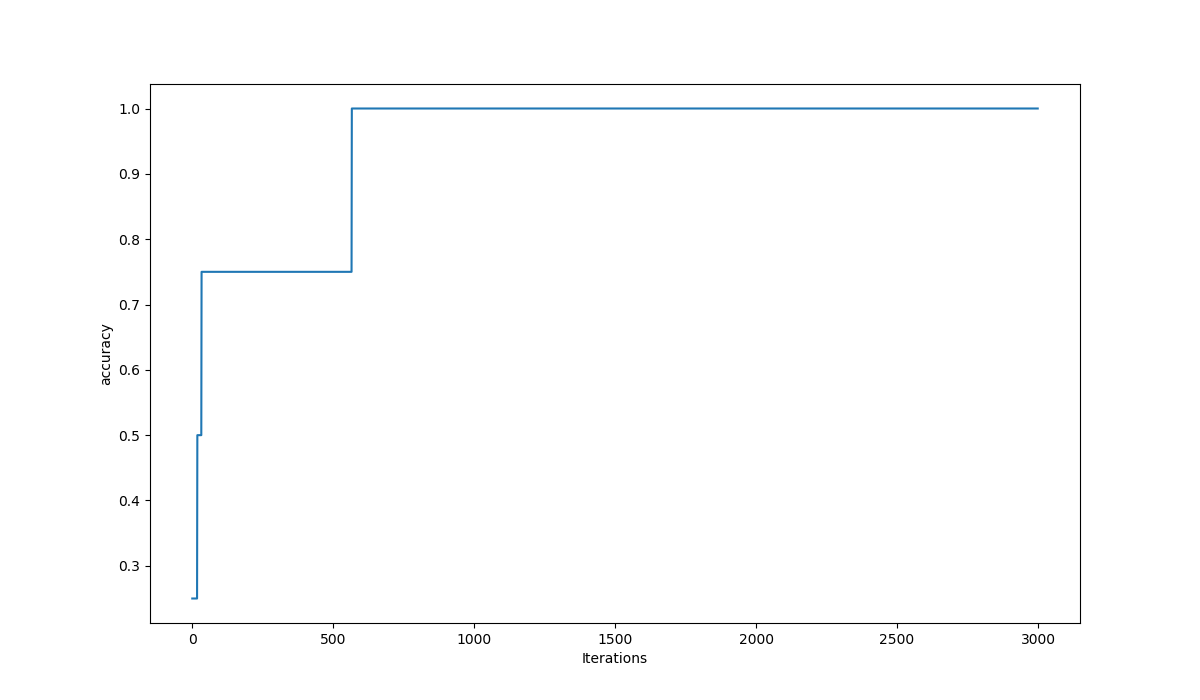
\includegraphics[height=8cm]{./nn_and.png}

\section*{OR}

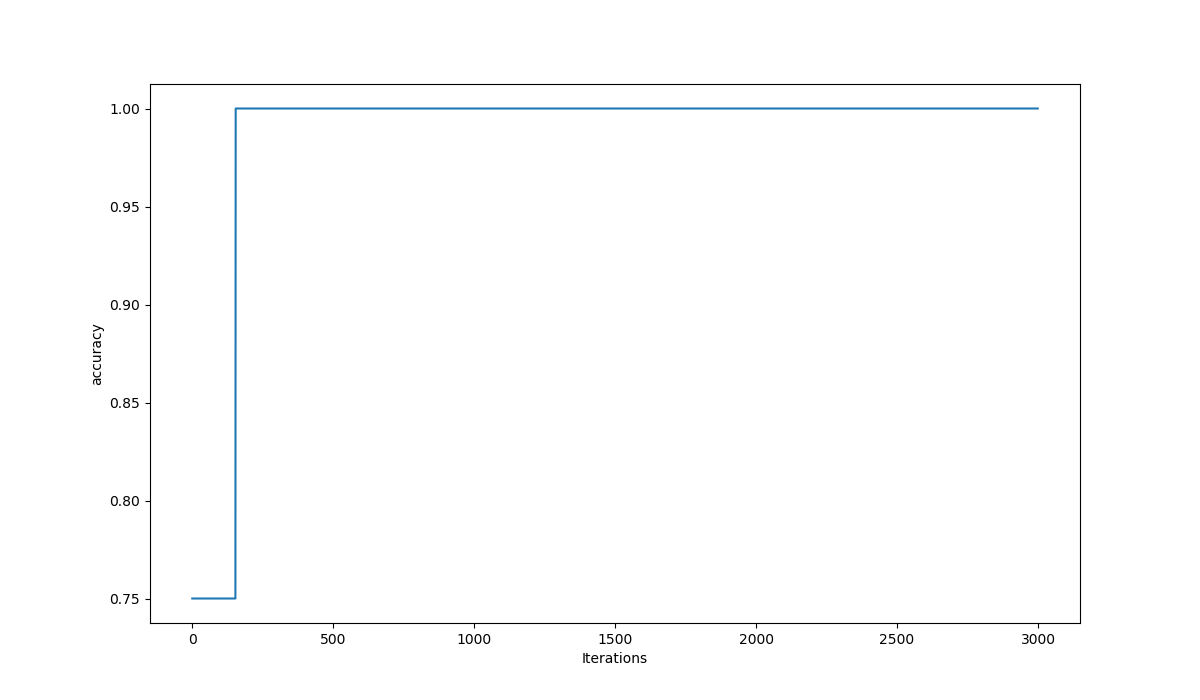
\includegraphics[height=8cm]{./nn_or.png}

\section*{XOR}

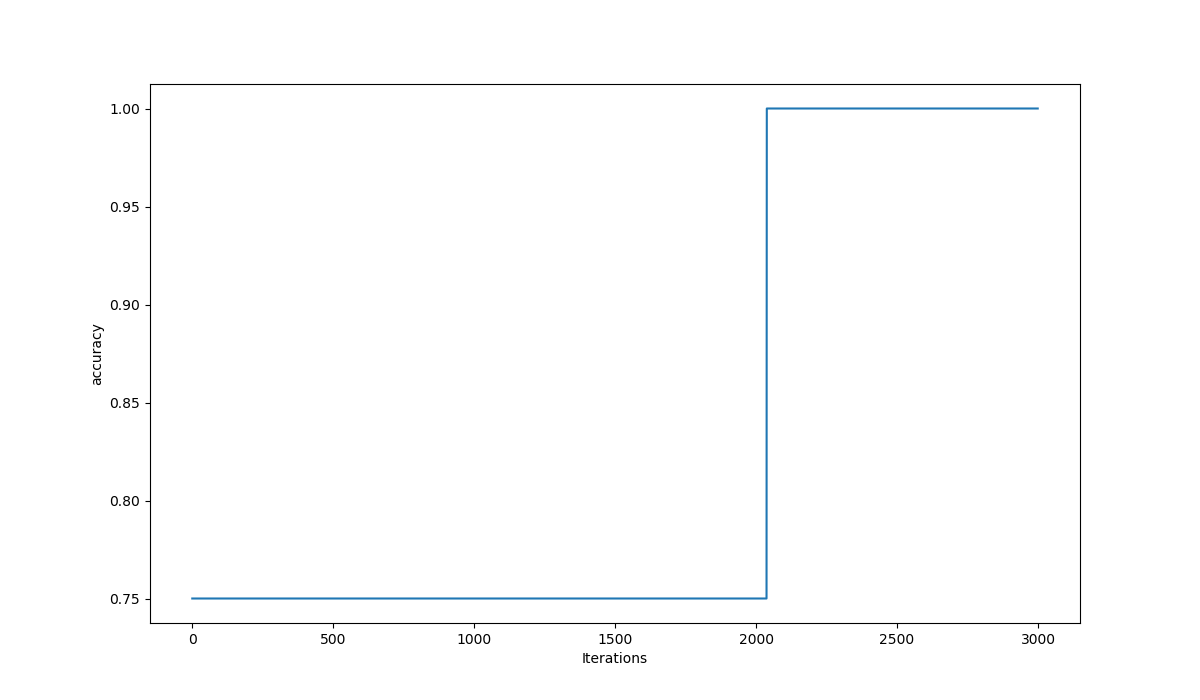
\includegraphics[height=8cm]{./nn_xor.png}


\section*{Erklärung des Codes}
Diesmal gibt es extrem wenig zu erklären, da das meiste Code von der Vorlesung / Tutorial
1 zu 1 genommen wurde und die Matritzenmultiplikationen in python geschrieben wurden. Nur eine Transponierung
hat gefehlt in den Formeln, dazu kommen wir nocht.

\section*{Fit Methode}

Interessant hier wäre vielleicht, dass wir den Datensatz in Batches mit je 7000 Beispiele unterteilen, sonst
können wir von den großen Datensatz gar nicht lernen. Adaptive Lernrate hat uns in dem Beispiel nicht geholfen,
wahrscheinlich war die Fehler kleiner wird und damit auch ihre Ableitung, wir korrigieren mit der Zeit immer
weniger. Weiter plotten wir nur den Score innerhalb des Batches und nicht das globale auf dem ganzen Trainingssatz.
Deswegen sieht man auch, dass den Score nach je Batch etwas senkt.

Es gibt nur zwei Unterschiede von den gegebenen Formeln. Erstens haben wir keine Diagonalmatrix benutzt,
aber das selbe mit Skalarprodukt erreicht. Der Grund war, dass wir für je Output eine Matrix bekommen, und diese man
in den Diagonalen einer weiteren Matrtitze nicht darstellen kann. \\ \\

Die zweite Unterschied ist, dass wir für die Berechnung der Delta (Backpropagated error) die transponierte
Gewichtsmatrix benutzt haben.

\begin{lstlisting}[style=py]
        def fit(self, X, y):
        self.history = []
        self.unique_labels = np.unique(y)
        X_ = self.data_normalizer.fit_transform(X)
        y_ = self.transform_y(y)
        self.W1 = np.vstack((
            np.random.randn(len(X_[0]), self.size_hidden),
            np.ones(self.size_hidden)))
        self.W2 = np.vstack((
            np.random.randn(self.size_hidden, self.size_output),
            np.ones(self.size_output)))

        batch_size = self.batch_size
        print('#Batches: {}'.format(math.ceil(len(X_) / batch_size)))
        print('#Iterations per batch: {}'.format(self.max_iterations))
        for batch_start in range(0, len(X_), batch_size):
            Xb = X_[batch_start:batch_start + batch_size]
            yb = y_[batch_start:batch_start + batch_size]
            for i in range(self.max_iterations):
                o_, o1, o1_, o2, o2_ = self.feed_forward(Xb)
                W2_ = self.W2[:-1]
                d1 = NN.sigmoid_derived(o1) # not diagonal matrix as in lecture, because sigmoid_derived(o1) is a vector
                d2 = NN.sigmoid_derived(o2)
                e = o2 - yb
                delta2 = d2 * e
                # transposing of the weights matrix missing in formula in lecture/tutorial of professor
                delta1 = d1 * (delta2.dot(W2_.T))
                deltaW2 = (-self.learning_rate * (delta2.T.dot(o1_))).T
                deltaW1 = (-self.learning_rate * delta1.T.dot(o_)).T
                self.W1 += deltaW1
                self.W2 += deltaW2

                # self.learning_rate = self.learning_rate * 1 / (1 + 0.0001 * i)

                if self.print_score_per_bach:
                    self.history.append(np.mean(self.unique_labels[o2.argmax(1)] == self.unique_labels[yb.argmax(1)]))
                else:
                    self.history.append(self.score(X, y))

            print('Batch #{} completed!'.format(math.floor(batch_start / batch_size) + 1))
\end{lstlisting}

\section*{Labels zu gewünschten Output}
Interessant ist vielleicht, dass wir von den Netz 10 Outputs haben für je Ziffer und diese müssen wir mit den
Labels vergleichen können. Dafür haben wir die folgende Methoden benutzt und damit auch die folgende Predict Methode.
Dabei nehmen wir das Output der letzten Schicht in dem Netz und wählen den Neuron mit der größten Wert. Danach
sollen wir dass wieder zu ein Label mappen, deswegen haben wir alle Mögliche Labels gespeichert.
In der transform\_y mappen wir z.B. 4 zu \[0,0,0,1.0,0,0,0,0\]

\begin{lstlisting}[style=py]
ef transform_y(self, y):
        y_ = np.zeros((len(y), len(self.unique_labels)))
        y_in_unique = np.vectorize(lambda x: list(self.unique_labels).index(x))(y)
        y_[range(len(y)), y_in_unique] = 1
        return y_

    def predict(self, X):
        X = self.data_normalizer.transform(X)
        return self.predict_(X)

    def predict_(self, X):
        o2 = self.feed_forward(X)[3]
        return self.unique_labels[o2.argmax(1)]
\end{lstlisting}


\section*{Sigmoid-Funktion und ihre Ableitung}

\begin{lstlisting}[style=py]
@staticmethod
    def sigmoid(x):
        return 1 / (1 + np.exp(-x))

    @staticmethod
    def sigmoid_derived(x):
        return x*(1-x)
\end{lstlisting}

\section*{Vollständiges Code boolean\_functions\_nn.py}

\begin{lstlisting}[style=py]
import numpy as np
from NN import NN


X = np.array([
    [0,0],
    [0,1],
    [1,0],
    [1,1]
])
y_and = np.array([a & b for a,b in X])
y_or  = np.array([a | b for a,b in X])
y_xor = np.array([a ^ b for a,b in X])

# AND
nn = NN(max_iterations=3000, size_hidden=10, size_output=2, learning_rate=0.01)
nn.fit(X, y_and)
nn.plot_accuracies('./nn_and.png')
print('Score and: {}'.format(nn.score(X, y_and)))

# OR
nn = NN(max_iterations=3000, size_hidden=10, size_output=2, learning_rate=0.01)
nn.fit(X, y_or)
nn.plot_accuracies('./nn_or.png')
print('Score or: {}'.format(nn.score(X, y_or)))

# XOR
nn = NN(max_iterations=3000, size_hidden=10, size_output=2, learning_rate=0.01)
nn.fit(X, y_and)
nn.plot_accuracies('./nn_xor.png')
print('Score xor: {}'.format(nn.score(X, y_and)))

\end{lstlisting}

\section*{Vollständiges Code digits\_small\_nn.py}

\begin{lstlisting}[style=py]
from Parser import get_data_set
from NN import NN


X_train, X_test, y_train, y_test = get_data_set('digits.data')
nn = NN()
nn.fit(X_train, y_train)
nn.plot_accuracies()
print('Score train: {}'.format(nn.score(X_train, y_train)))
print('Score: {}'.format(nn.score(X_test, y_test)))

\end{lstlisting}

\section*{Vollständiges Code digits\_big\_nn.py}

\begin{lstlisting}[style=py]
from sklearn.datasets import fetch_mldata
from sklearn.model_selection import train_test_split
import numpy as np
from NN import NN

print('fetching data-set')
mnist = fetch_mldata('mnist-original', data_home='./Dataset/mnist.pkl/mnist_dataset/')
print('MNIST original fetched')
X = np.array(mnist.data, dtype=np.float64)
y = mnist.target
X_train, X_test, y_train, y_test = train_test_split(X, y, train_size=0.7, test_size=0.3,
                                                        random_state=1)


nn = NN(max_iterations=250, print_score_per_bach=True, batch_size=1000)
nn.fit(X_train, y_train)
nn.plot_accuracies('./20_inner_big.png')
print('Score train: {}'.format(nn.score(X_train, y_train)))
print('Score: {}'.format(nn.score(X_test, y_test)))

\end{lstlisting}

\section*{Vollständiges Code DataNormalizer.py (von Musterlösung genommen und etwas angepasst)}

\begin{lstlisting}[style=py]
import numpy as np

class DataNormalizer:
    def fit(self, X):
        self.mean = np.mean(X, axis=0)
        self.var = np.var(X, axis=0) + np.nextafter(0, 1)

    def transform(self, X):
        return (X - self.mean) / self.var

    def fit_transform(self, X):
        self.fit(X)
        return self.transform(X)
\end{lstlisting}

\section*{Vollständiges Code NN.py}

\begin{lstlisting}[style=py]
from Classifier import Classifier
from DataNormalizer import DataNormalizer
import numpy as np
from matplotlib import pyplot as plt
import math


class NN(Classifier):
    def __init__(self, max_iterations=3000, learning_rate=0.0020,
                 size_hidden=20, size_output=10, print_score_per_bach=False, batch_size=7000):
        self.data_normalizer = DataNormalizer()
        self.size_hidden = size_hidden
        self.size_output = size_output
        self.max_iterations = max_iterations
        self.learning_rate = learning_rate
        self.print_score_per_bach = print_score_per_bach
        self.W1 = None
        self.W2 = None
        self.unique_labels = None
        self.batch_size = batch_size

    def fit(self, X, y):
        self.history = []
        self.unique_labels = np.unique(y)
        X_ = self.data_normalizer.fit_transform(X)
        y_ = self.transform_y(y)
        self.W1 = np.vstack((
            np.random.randn(len(X_[0]), self.size_hidden),
            np.ones(self.size_hidden)))
        self.W2 = np.vstack((
            np.random.randn(self.size_hidden, self.size_output),
            np.ones(self.size_output)))

        batch_size = self.batch_size
        print('#Batches: {}'.format(math.ceil(len(X_) / batch_size)))
        print('#Iterations per batch: {}'.format(self.max_iterations))
        for batch_start in range(0, len(X_), batch_size):
            Xb = X_[batch_start:batch_start + batch_size]
            yb = y_[batch_start:batch_start + batch_size]
            for i in range(self.max_iterations):
                o_, o1, o1_, o2, o2_ = self.feed_forward(Xb)
                W2_ = self.W2[:-1]
                d1 = NN.sigmoid_derived(o1) # not diagonal matrix as in lecture, because sigmoid_derived(o1) is a vector
                d2 = NN.sigmoid_derived(o2)
                e = o2 - yb
                delta2 = d2 * e
                # transposing of the weights matrix missing in formula in lecture/tutorial of professor
                delta1 = d1 * (delta2.dot(W2_.T))
                deltaW2 = (-self.learning_rate * (delta2.T.dot(o1_))).T
                deltaW1 = (-self.learning_rate * delta1.T.dot(o_)).T
                self.W1 += deltaW1
                self.W2 += deltaW2

                # self.learning_rate = self.learning_rate * 1 / (1 + 0.0001 * i)

                if self.print_score_per_bach:
                    self.history.append(np.mean(self.unique_labels[o2.argmax(1)] == self.unique_labels[yb.argmax(1)]))
                else:
                    self.history.append(self.score(X, y))

            print('Batch #{} completed!'.format(math.floor(batch_start / batch_size) + 1))

    def feed_forward(self, X):
        o_ = np.c_[X, np.ones(len(X))]
        o1 = NN.sigmoid(o_.dot(self.W1))
        o1_ = np.c_[o1, np.ones(len(o1))]
        o2 = NN.sigmoid(o1_.dot(self.W2))
        o2_ = np.c_[o2, np.ones(len(o2))]

        return o_, o1, o1_, o2, o2_

    @staticmethod
    def sigmoid(x):
        return 1 / (1 + np.exp(-x))

    @staticmethod
    def sigmoid_derived(x):
        return x*(1-x)

    def transform_y(self, y):
        y_ = np.zeros((len(y), len(self.unique_labels)))
        y_in_unique = np.vectorize(lambda x: list(self.unique_labels).index(x))(y)
        y_[range(len(y)), y_in_unique] = 1
        return y_

    def predict(self, X):
        X = self.data_normalizer.transform(X)
        return self.predict_(X)

    def predict_(self, X):
        o2 = self.feed_forward(X)[3]
        return self.unique_labels[o2.argmax(1)]

    def plot_accuracies(self, file_name=None):
        plt.figure(figsize=(12, 7))
        plt.plot(self.history)
        plt.xlabel("Iterations")
        plt.ylabel("accuracy")

        if file_name is None:
            plt.show()
        else:
            plt.savefig(file_name)

\end{lstlisting}

\section*{Vollständiges Code NeuralNetwork.py}

\begin{lstlisting}[style=py]
from Classifier import Classifier
from DataNormalizer import DataNormalizer
import numpy as np
from matplotlib import pyplot as plt
from Parser import get_data_set


class NeuralNetwork(Classifier):
    def __init__(self, layers=None, max_iterations=3000, learning_rate=0.0025):
        """

        :param layers: tuple defining the amount of neurons to be used pro layers, thereby defining the network
        :param max_iterations:
        :param learning_rate:
        """
        self.data_normalizer = DataNormalizer()
        self.W_ext = None
        self.max_iterations = max_iterations
        self.learning_rate = learning_rate
        self.layers = layers
        self.history = []

        if self.layers is None:
            self.k_layers = 3
        else:
            self.k_layers = len(self.layers)

    def transform_y(self, y):
        y_ = np.zeros((len(y), len(self.unique_labels)))
        y_in_unique = np.vectorize(lambda x: list(self.unique_labels).index(x))(y)
        y_[range(len(y)), y_in_unique] = 1
        return y_

    def fit(self, X, y):
        self.unique_labels = np.unique(y)
        X_ = self.data_normalizer.fit_transform(X)
        y_ = self.transform_y(y)

        if self.layers is not None:
            self.W_ext = np.array([np.random.randn(len(X_[0] + 1, self.layers[i])) if i == 0 else
                                   np.random.randn(self.layers[i - 1] + 1, self.layers[i])
                                   for i in self.layers])
        else:
            self.W_ext = np.array([np.random.randn(len(X_[0]) + 1, 20), np.random.randn(20 + 1, 15),
                                   np.random.randn(15+1, 10)])

        batch_size = 1000
        for batch_start in range(0, len(X_), batch_size):
            Xb = X_[batch_start:batch_start + batch_size + 1]
            yb = y_[batch_start:batch_start + batch_size + 1]
            for it in range(self.max_iterations):
                O_s = self.get_O_s(Xb)
                D_s = [(o * (1.0 - o)) for o in O_s[2::2]]
                e = (O_s[-1] - yb)
                der_e_s = self.get_der_e_s(D_s, e)
                delta_W_ext = self.get_delta_W_ext(der_e_s, O_s[::2])

                for i, delta in enumerate(delta_W_ext):
                    self.W_ext[i] += delta

                self.history.append(self.score(X, y))

    @staticmethod
    def add_ones(X):
        return np.c_[np.ones(len(X)), X]

    @staticmethod
    def sigmoid(x):
        return 1 / (1 + np.exp(-x))

    def get_O_s(self, X):
        O_s = [X]
        for i in range(self.k_layers):
            O_i_minus_1 = np.c_[O_s[-1], np.ones(len(X))]  # extend to get o(i-1)^
            O_s.append(O_i_minus_1)
            O_i = NeuralNetwork.sigmoid(O_i_minus_1.dot(self.W_ext[i]))
            O_s.append(O_i)

        return O_s

    def get_der_e_s(self, D_s, e):
        W = [w[1:] for w in self.W_ext]
        der_e_l = e * D_s[-1]
        der_e_s = [der_e_l]

        for i in range(self.k_layers - 1):
            der_e_i = D_s[-i - 2] * (der_e_s[0]).dot(W[-i - 1].T)
            der_e_s = [der_e_i] + der_e_s

        return der_e_s

    def get_delta_W_ext(self, der_e_s, O_s):
        delta_W_ext = []

        for i in range(self.k_layers):
            o_i_ext = np.c_[O_s[i], np.ones(len(O_s[i]))]
            delta_W_i = der_e_s[i].T.dot(o_i_ext)
            delta_W_ext.append(delta_W_i.T)

        return np.array(delta_W_ext) * -self.learning_rate

    def predict(self, X):
        X = self.data_normalizer.transform(X)
        return self.predict_(X)

    def predict_(self, X):
        O_s = self.get_O_s(X)
        results = O_s[-1]
        return self.unique_labels[results.argmax(1)]

    def plot_accuracies(self, file_name=None):
        plt.figure(figsize=(12, 7))
        plt.plot(self.history)
        plt.xlabel("Iterations")
        plt.ylabel("accuracy")

        if file_name is None:
            plt.show()
        else:
            plt.savefig(file_name)


X_train, X_test, y_train, y_test = get_data_set('digits.data')
nn = NeuralNetwork()
nn.fit(X_train, y_train)
nn.plot_accuracies('./2_hidden_layers_20_15_with_7_batches.png')
print('Score train: {}'.format(nn.score(X_train, y_train)))
print('Score: {}'.format(nn.score(X_test, y_test)))

\end{lstlisting}

% /////////////////////// END DOKUMENT /////////////////////////
\end{document}
